\documentclass[tikz,border=2pt]{standalone}
\usepackage{amsmath}
\usepackage{siunitx}
\usetikzlibrary{shapes,arrows,positioning,fit,calc}

\begin{document}
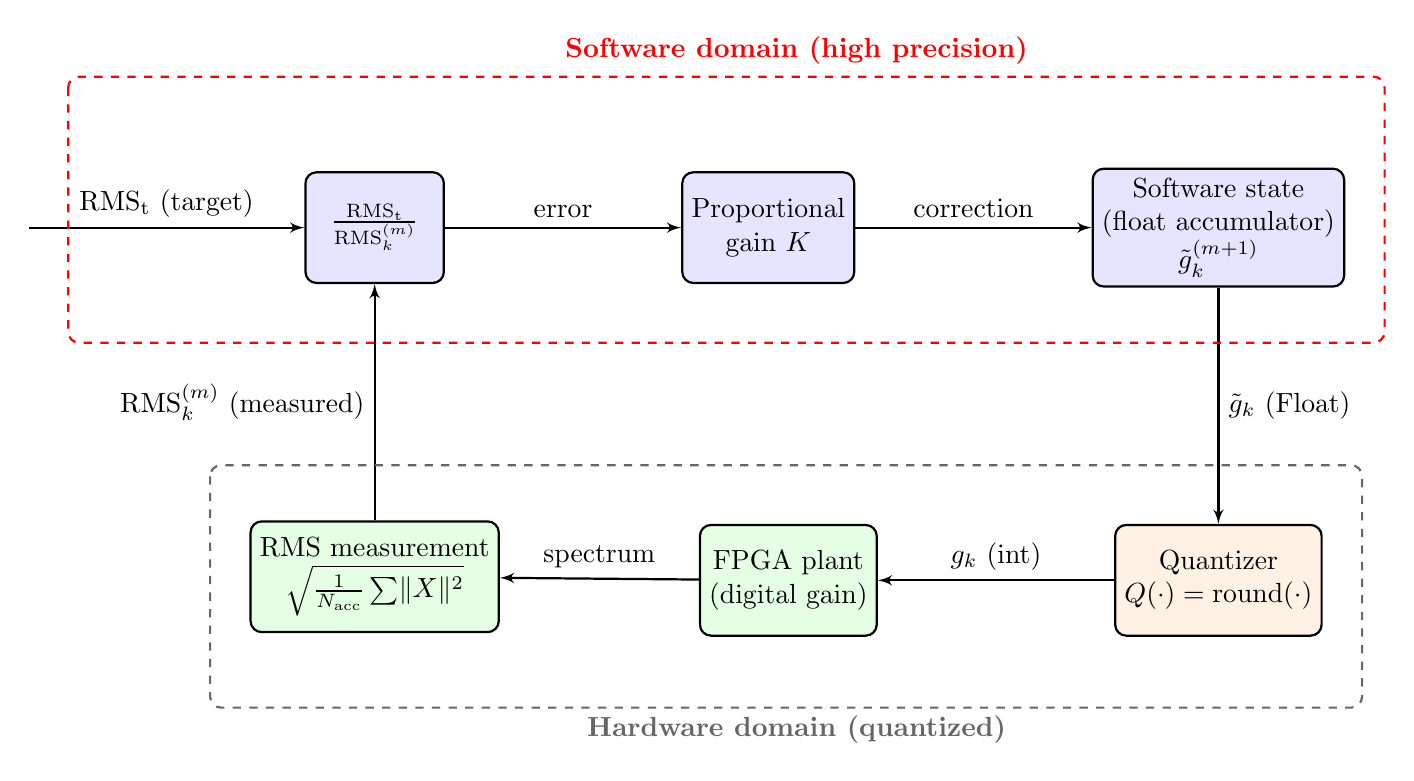
\begin{tikzpicture}[auto, node distance=2cm,>=latex', thick]
    % Estilos para los bloques
    \tikzstyle{block} = [draw, rectangle, fill=blue!10, minimum height=4em, minimum width=5em, align=center, rounded corners]
    \tikzstyle{hwblock} = [draw, rectangle, fill=green!10, minimum height=4em, minimum width=5em, align=center, rounded corners]
    \tikzstyle{qblock} = [draw, rectangle, fill=orange!10, minimum height=4em, minimum width=5em, align=center, rounded corners]
    \tikzstyle{input} = [coordinate]
    \tikzstyle{output} = [coordinate]

    % --- Nodos del Dominio de Software ---
    \node [input, name=input_pt] {};
    % Aumentamos la distancia para evitar solapamiento con las entradas
    \node [block, right=3.5cm of input_pt] (ratio) {$\frac{\text{RMS}_\mathrm{t}}{\text{RMS}_k^{(m)}}$};
    % Aumentamos la distancia entre bloques
    \node [block, right=3cm of ratio] (controller) {Proportional\\ gain $K$};
    \node [block, right=3cm of controller, minimum width=7em] (software) {Software state\\ (float accumulator)\\ $\tilde{g}_k^{(m+1)}$};

    % --- Nodos del Dominio de Hardware ---
    % Colocamos el cuantizador debajo del estado de software
    \node [qblock, below=3cm of software] (quantizer) {Quantizer\\ $Q(\cdot) = \text{round}(\cdot)$};
    \node [hwblock, left=3cm of quantizer] (fpga) {FPGA plant\\ (digital gain)};
    \node [hwblock, below=3cm of ratio] (rms) {RMS measurement\\[0.3em]
        $\sqrt{\frac{1}{N_\text{acc}} \sum \lVert X \rVert^2}$};

    % --- Conexiones ---
    % Entradas al Ratio Calc
    \draw [->] (input_pt) -- node[above] {$\text{RMS}_\mathrm{t}$ (target)} (ratio.west);
    % Realimentación desde RMS a Ratio Calc (ruta ortogonal clara)
    \draw [->] (rms.north) -- node[left] {$\text{RMS}_k^{(m)}$ (measured)} (ratio.south);

    % Ruta de Software
    \draw [->] (ratio) -- node[above] {error} (controller);
    \draw [->] (controller) -- node[above] {correction} (software);

    % Conexión Software a Hardware
    \draw [->] (software) -- node[right] {$\tilde{g}_k$ (Float)} (quantizer);

    % Ruta de Hardware
    \draw [->] (quantizer) -- node[above] {$g_k$ (int)} (fpga);
    \draw [->] (fpga) -- node[above] {spectrum} (rms);


    % --- Cajas de Dominio ---
    % Dominio de Software (Rojo, punteado)
    % Usamos coordenadas relativas a los nodos extremos con un margen
    \draw[red, dashed, thick, rounded corners]
        ($(ratio.north west)+(-3.0, 1.2)$) rectangle ($(software.south east)+(0.5, -0.7)$);
    \node[red, above, font=\bfseries] at ($(ratio.north)!0.5!(software.north)+(0, 1.2)$) {Software domain (high precision)};

    % Dominio de Hardware (Gris, punteado)
    \draw[black!60, dashed, thick, rounded corners]
        ($(rms.north west)+(-0.5, 0.7)$) rectangle ($(quantizer.south east)+(0.5, -0.9)$);
    \node[black!60, below, font=\bfseries] at ($(rms.south)!0.5!(quantizer.south)+(0, -0.9)$) {Hardware domain (quantized)};

\end{tikzpicture}
\end{document}